\documentclass[11pt]{article}
\usepackage{geometry,marginnote} % Pour passer au format A4
\geometry{hmargin=1cm, vmargin=1cm} % 

% Page et encodage
\usepackage[T1]{fontenc} % Use 8-bit encoding that has 256 glyphs
\usepackage[english,french]{babel} % Français et anglais
\usepackage[utf8]{inputenc} 

\usepackage{lmodern,numprint}
\setlength\parindent{0pt}

% Graphiques
\usepackage{graphicx,float,grffile,units}
\usepackage{tikz,pst-eucl,pst-plot,pstricks,pst-node,pstricks-add,pst-fun,pgfplots} 

% Maths et divers
\usepackage{amsmath,amsfonts,amssymb,amsthm,verbatim}
\usepackage{multicol,enumitem,url,eurosym,gensymb,tabularx}

\DeclareUnicodeCharacter{20AC}{\euro}



% Sections
\usepackage{sectsty} % Allows customizing section commands
\allsectionsfont{\centering \normalfont\scshape}

% Tête et pied de page
\usepackage{fancyhdr} \pagestyle{fancyplain} \fancyhead{} \fancyfoot{}

\renewcommand{\headrulewidth}{0pt} % Remove header underlines
\renewcommand{\footrulewidth}{0pt} % Remove footer underlines

\newcommand{\horrule}[1]{\rule{\linewidth}{#1}} % Create horizontal rule command with 1 argument of height

\newcommand{\Pointilles}[1][3]{%
  \multido{}{#1}{\makebox[\linewidth]{\dotfill}\\[\parskip]
}}

\newtheorem{Definition}{Définition}

\usepackage{siunitx}
\sisetup{
    detect-all,
    output-decimal-marker={,},
    group-minimum-digits = 3,
    group-separator={~},
    number-unit-separator={~},
    inter-unit-product={~}
}

\setlength{\columnseprule}{1pt}

\begin{document}

\horrule{2px}
\section*{Chapitre 4 - Nombres relatifs}
\horrule{2px}

\subsection*{Connaissances de cours}

\begin{enumerate}
  \item[1.] Nombres négatifs : \dotfill
  \item[2.] Nombres opposés \dotfill
\end{enumerate}

\subsection*{Exercices sur les nombres}

\begin{multicols}{2}

  \textit{Écrire la soustraction et le nombre négatif correspondant}

  \begin{enumerate}
    \item[1.] $  -4 = $ \dotfill
    \item[2.] $-120 = $ \dotfill
    \item[3.] $-0,4 = $ \dotfill
    \item[4.] $-\pi = $ \dotfill
    \item[5.] $ -\frac{1}{3} = $ \dotfill
    \item[6.] $= 0 - 10$  \dotfill
    \item[7.] $= 0 - \SI{0,42}{}$  \dotfill
    \item[8.] $= 0 - \SI{52000}{}$  \dotfill   
  \end{enumerate}
  \columnbreak

  \textit{Écrire l'opposé et écrire l'opération correspondante.}

  \begin{enumerate}
    \item[1.] L'opposé de $4$ est \dots \dots car \dotfill
    \item[2.] L'opposé de $-6$ est \dots \dots car \dotfill
    \item[3.] L'opposé de $\SI{25400}{}$ est \dots \dots car \dotfill
    \item[4.] L'opposé de $\SI{-0,5}{}$ est \dots \dots car \dotfill
    \item[5.] L'opposé de $\pi$ est \dots \dots car \dotfill
    \item[6.] L'opposé de $\dfrac{2}{3}$ est \dots \dots car \dotfill
  \end{enumerate}

\end{multicols}

\subsection*{Exercice sur les comparaisons}

\textit{Ranger par ordre croissant ou décroissant. Utiliser }$>$ \textit{ et } $<$.

\begin{enumerate}
  \item[1.] 0; -1; 2; -3; 4; -5
  \item[2.] 12; -10; \SI{1,2}{} ; \SI{-1,4}{} ; \SI{-1,5}{} , \SI{-1,25}{} 
  \item[3.] -200 ; 250 ; \SI{-3000}{} ; -450 ; 0,5 ; 120
\end{enumerate}

\subsection*{Exercice sur la droite graduée}

\textit{Placer les points sur sur la bonne graduation de la droite graduée.}

$A = 3 ; B = -2 ; C = \SI{2,5}{} ; D = \SI{-3,5}{} ; E = \SI{-0,5}{}$

\begin{figure}[H]
  \centering
  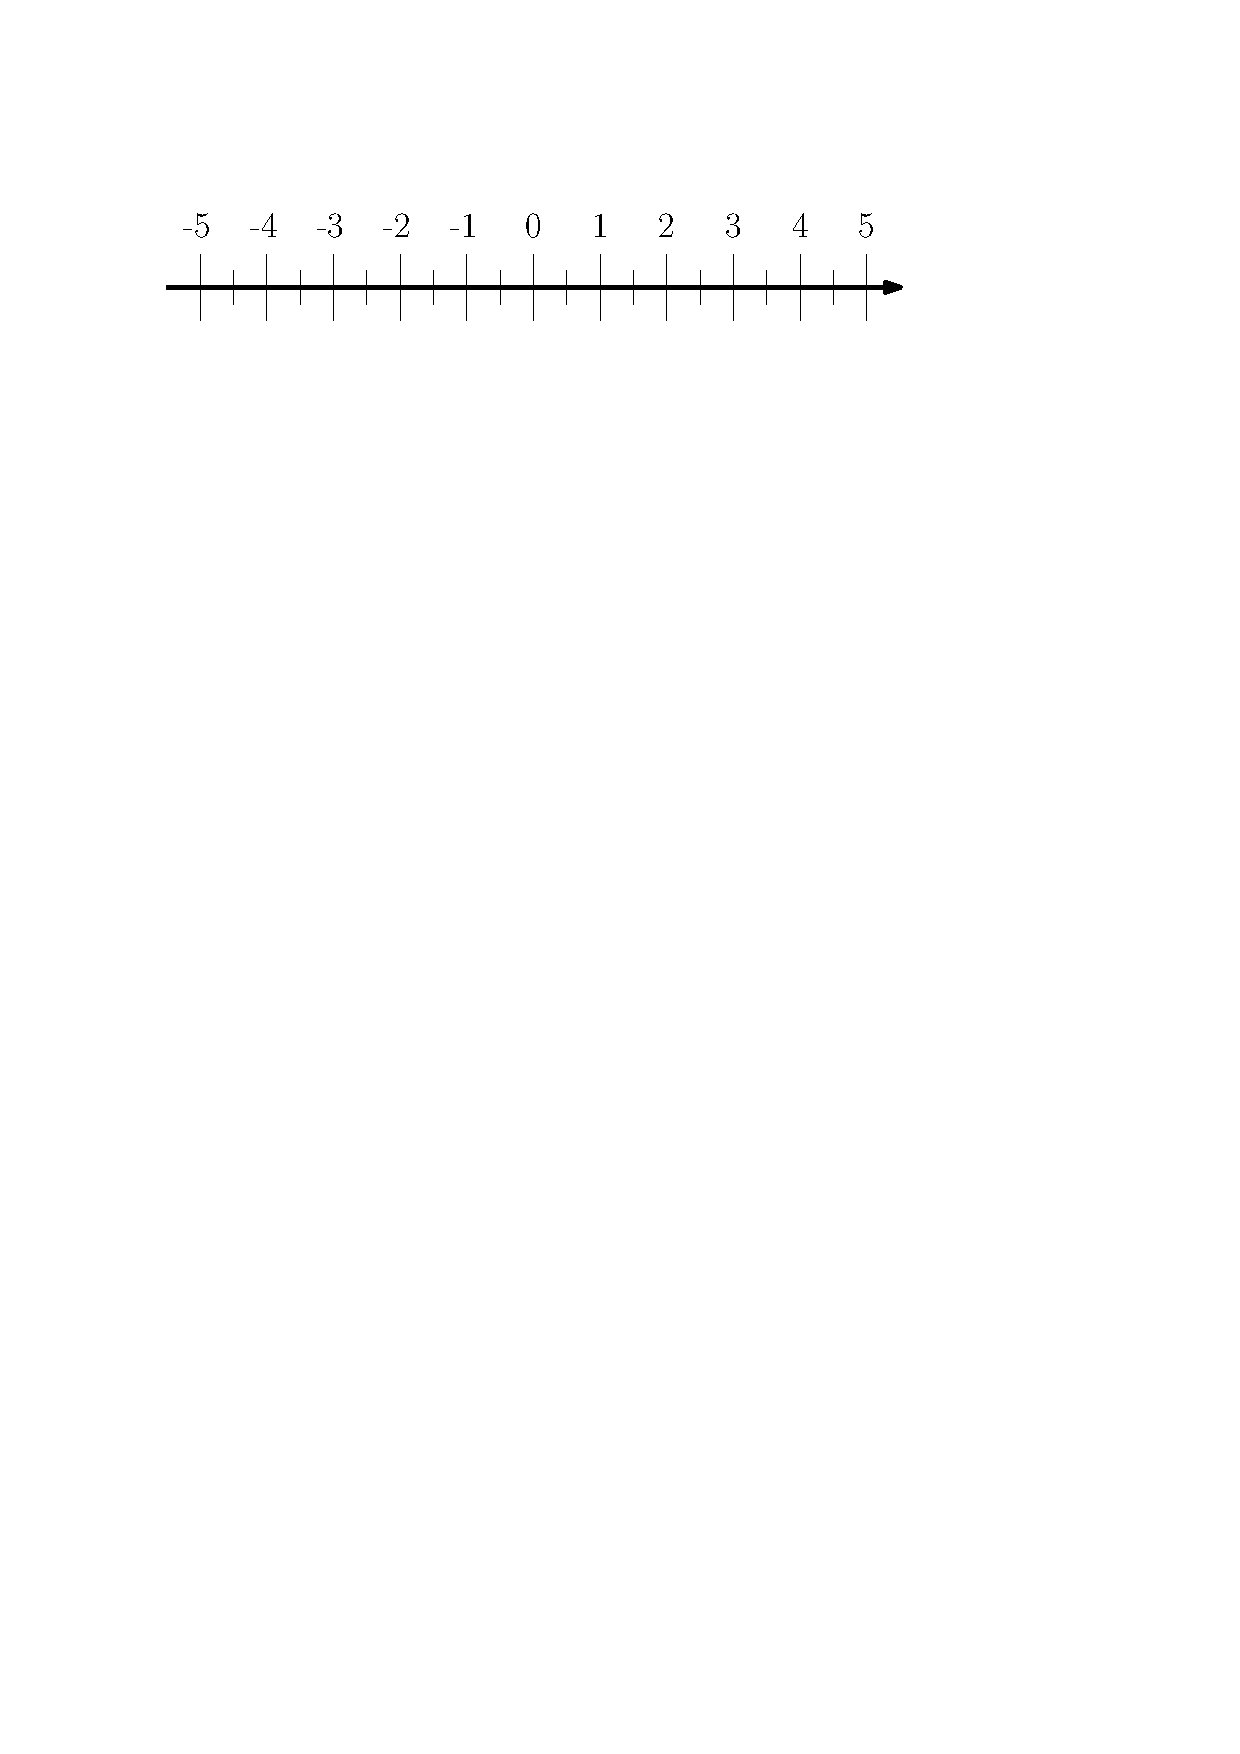
\includegraphics[width=0.9\linewidth]{5x4-relatifs/c-axe-1.pdf}
\end{figure}

$A = \SI{2,5}{} ; B = \SI{-2,25}{} ; C = \SI{3,75}{} ; D = \SI{-3,2}{} ; E = \SI{-0,7}{}$

\begin{figure}[H]
  \centering
  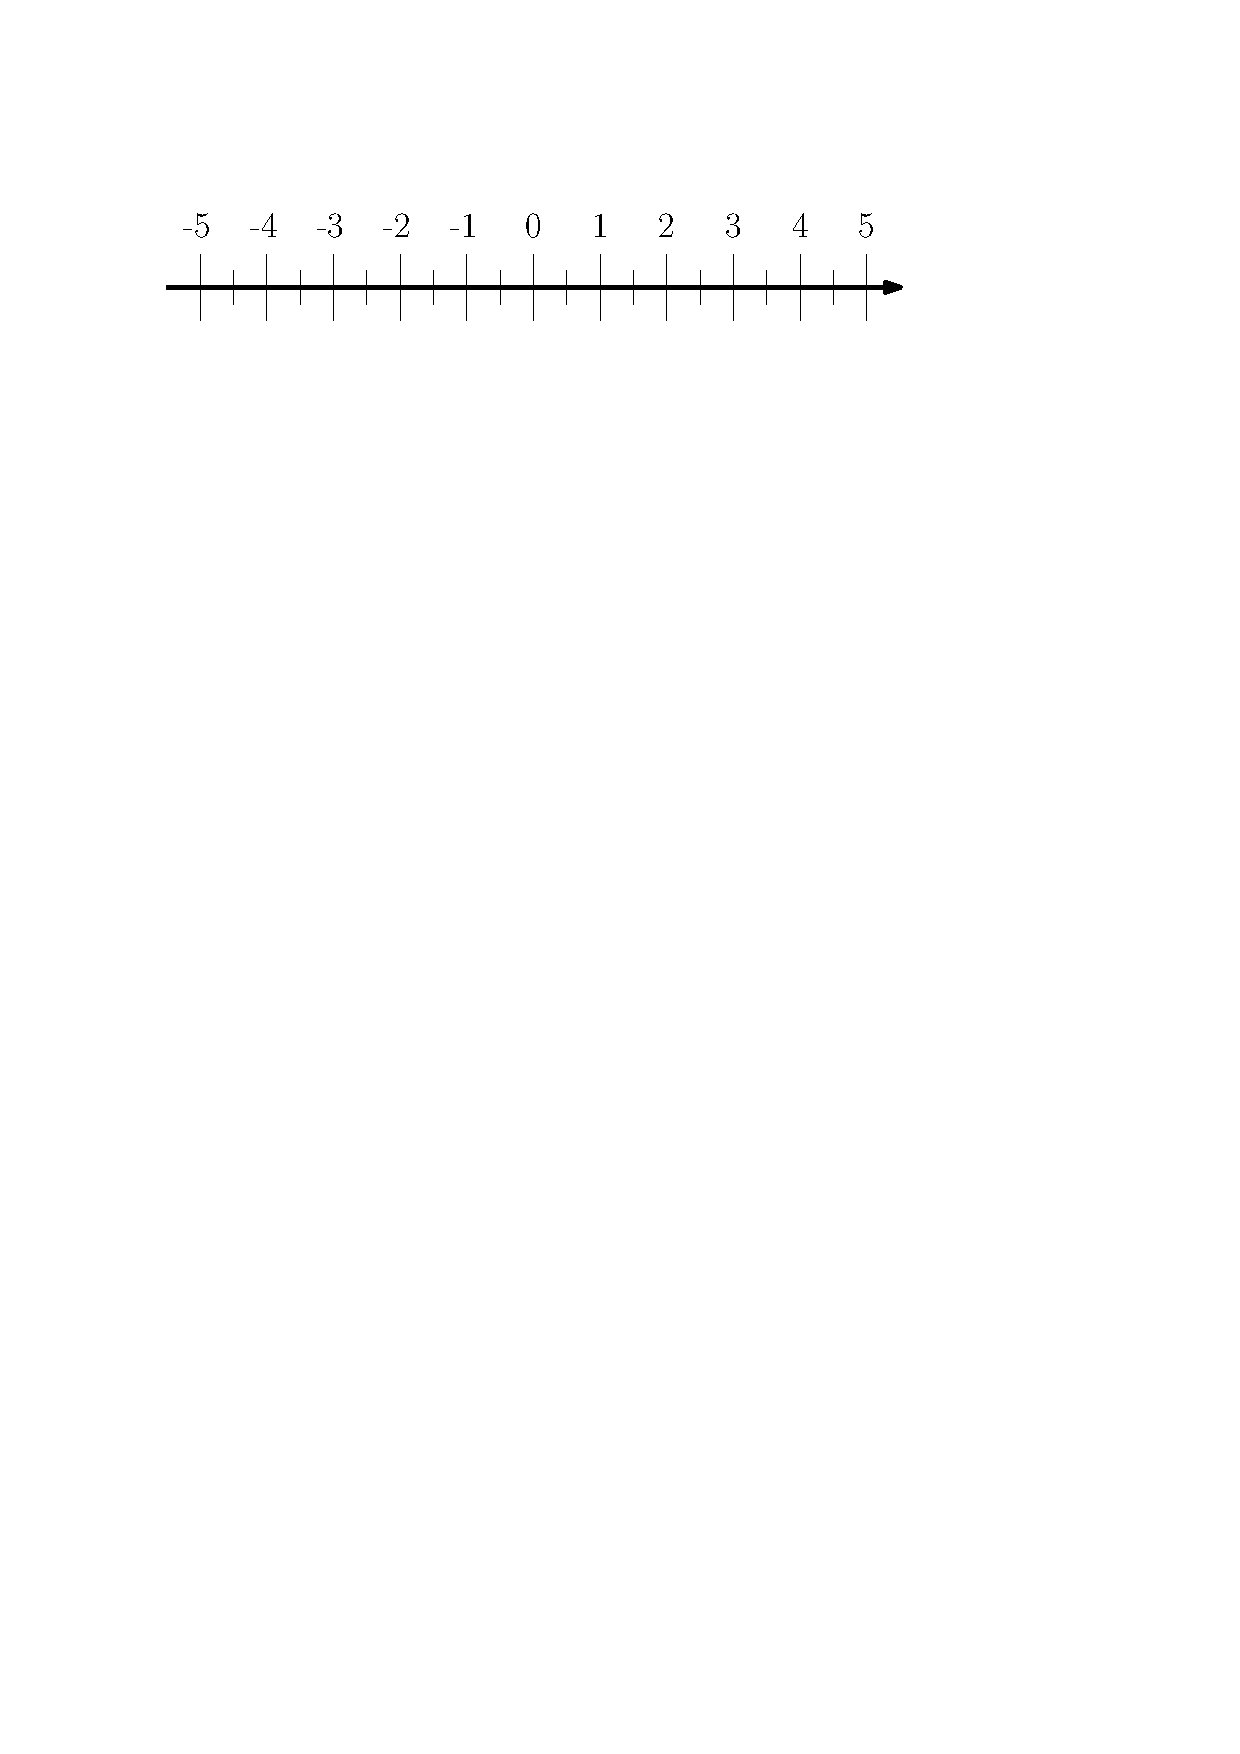
\includegraphics[width=0.9\linewidth]{5x4-relatifs/c-axe-1.pdf}
\end{figure}

\end{document}
